% preamble
\documentclass[aspectratio=169]{beamer}
\usetheme{Madrid}
\usecolortheme{orchid}
\usepackage{graphicx}
\usepackage{tikz}

% begin
\begin{document}
% title page
\title{DecryptZero}
\author[Premchander]{Kanishk Premchander}
\institute[ICR Portland 2024]{Institute for Computing in Research}
\date[08/01/2024]{August 1, 2024}

\frame{\titlepage}

% section 1 - backstory
\section{Backstory}

\begin{frame}{Backstory} \pause
    \begin{figure}
        \centering
        \includegraphics[width=0.75\textwidth,keepaspectratio]{images/magnus-vs-hans.png}
        \caption{GM Magnus Carlsen vs GM Hans Niemann (Sinquefield Cup 2022)}
    \end{figure}
\end{frame}

\begin{frame}{Backstory} \pause
    \begin{figure}
        \centering
        \includegraphics<2>[height=0.75\textheight,keepaspectratio]{images/mistake-example.png}
        \includegraphics<3>[height=0.75\textheight,keepaspectratio]{images/mistake-example-1.png}
    \end{figure}
\end{frame}

\begin{frame}{Backstory}
    \begin{figure}
        \begin{minipage}{.5\textwidth}
            \begin{center}
                \includegraphics[height=0.75\textheight,keepaspectratio]{images/mistake-example-1.png}
            \end{center}
        \end{minipage}%
        \begin{minipage}{.5\textwidth}
            \begin{center}
                \includegraphics<1>[width=0.75\textwidth,keepaspectratio]{images/mistake-move-1.png}
                \includegraphics<2>[width=0.75\textwidth,keepaspectratio]{images/mistake-move-2.png}
                \includegraphics<3>[width=0.75\textwidth,keepaspectratio]{images/mistake-move-3.png}
            \end{center}
        \end{minipage}
    \end{figure}
\end{frame}

\begin{frame}{Backstory} \pause
    \begin{figure}
        \begin{center}
            \includegraphics<2>[height=0.75\textheight,keepaspectratio]{images/illegal-move-0.png}
            \includegraphics<3>[height=0.75\textheight,keepaspectratio]{images/illegal-move-1.png}
            \includegraphics<4>[height=0.75\textheight,keepaspectratio]{images/illegal-move-2.png}
            \includegraphics<5>[height=0.75\textheight,keepaspectratio]{images/illegal-move-3.png}
            \includegraphics<6>[height=0.75\textheight,keepaspectratio]{images/illegal-move-4.png}
            \caption{GM Sergey Zagrebelny vs GM Dmitry Kayumov (both IMs at the time)}
        \end{center}
    \end{figure}
\end{frame}

\begin{frame}{Backstory}
    \begin{figure}
        \begin{minipage}{.5\textwidth}
            \begin{center}
                \includegraphics<1>[width=0.75\textwidth,keepaspectratio]{images/illegal-move-0.png}
                \includegraphics<2>[width=0.75\textwidth,keepaspectratio]{images/illegal-move-1.png}
                \includegraphics<3>[width=0.75\textwidth,keepaspectratio]{images/illegal-move-2.png}
                \includegraphics<4>[width=0.75\textwidth,keepaspectratio]{images/illegal-move-3.png}
                \includegraphics<5>[width=0.75\textwidth,keepaspectratio]{images/illegal-move-4.png}
                \includegraphics<6>[width=0.75\textwidth,keepaspectratio]{images/real-move-5.png}
                \caption{Accepted Scoresheet Game}
            \end{center}
        \end{minipage}%
        \begin{minipage}{.5\textwidth}
            \begin{center}
                \includegraphics<1>[width=0.75\textwidth,keepaspectratio]{images/illegal-move-0.png}
                \includegraphics<2>[width=0.75\textwidth,keepaspectratio]{images/real-move-1.png}
                \includegraphics<3>[width=0.75\textwidth,keepaspectratio]{images/real-move-2.png}
                \includegraphics<4>[width=0.75\textwidth,keepaspectratio]{images/real-move-3.png}
                \includegraphics<5>[width=0.75\textwidth,keepaspectratio]{images/real-move-4.png}
                \includegraphics<6>[width=0.75\textwidth,keepaspectratio]{images/real-move-5.png}
                \caption{Actual Illegal Game}
            \end{center}
        \end{minipage}
    \end{figure}
\end{frame}

\begin{frame}{Backstory} \pause
    \begin{figure}
        \begin{tikzpicture}[overlay, remember picture]
            \node<2-> [anchor=north west, scale=2.0, xshift=1.2cm, yshift=-0.5cm]
                at (current page.north west) %left upper corner of the page
                {\includegraphics[width=5cm]{images/messy-example-1.png}};
            \node<3-> [anchor=north west, xshift=1.5cm, yshift=-1cm]
                at (current page.north west) %left upper corner of the page
                {\includegraphics[width=5cm]{images/messy-example-2.png}};
            \node<4-> [anchor=north west, xshift=7.5cm, yshift=-1cm]
                at (current page.north west) %left upper corner of the page
                {\includegraphics[width=5cm]{images/messy-example-3.png}};
            \node<5-> [anchor=north west, scale=1.5, xshift=1.5cm,  yshift=-0.75cm]
                at (current page.north west) %left upper corner of the page
                {\includegraphics[width=5cm]{images/messy-example-4.png}};
            \node<6-> [anchor=north west, xshift=6.5cm,  yshift=-1.0cm]
                at (current page.north west) %left upper corner of the page
                {\includegraphics[width=5cm]{images/messy-example-5.png}};
            \node<7-> [anchor=north west, xshift=2.5cm,  yshift=-1.0cm]
                at (current page.north west) %left upper corner of the page
                {\includegraphics[width=5cm]{images/messy-example-6.png}};
            \node<8-> [anchor=north west, scale=0.75, xshift=8cm,  yshift=-2.0cm]
                at (current page.north west) %left upper corner of the page
                {\includegraphics[width=5cm]{images/messy-example-7.png}};
        \end{tikzpicture}
    \end{figure}
\end{frame}

% section 2 - project intro
\section{The Project}

\begin{frame}{The Project}
    DecryptZero - an OCR model built to read chess notation \pause
    \begin{figure}
        \begin{minipage}{.33\textwidth}
            \begin{center}
                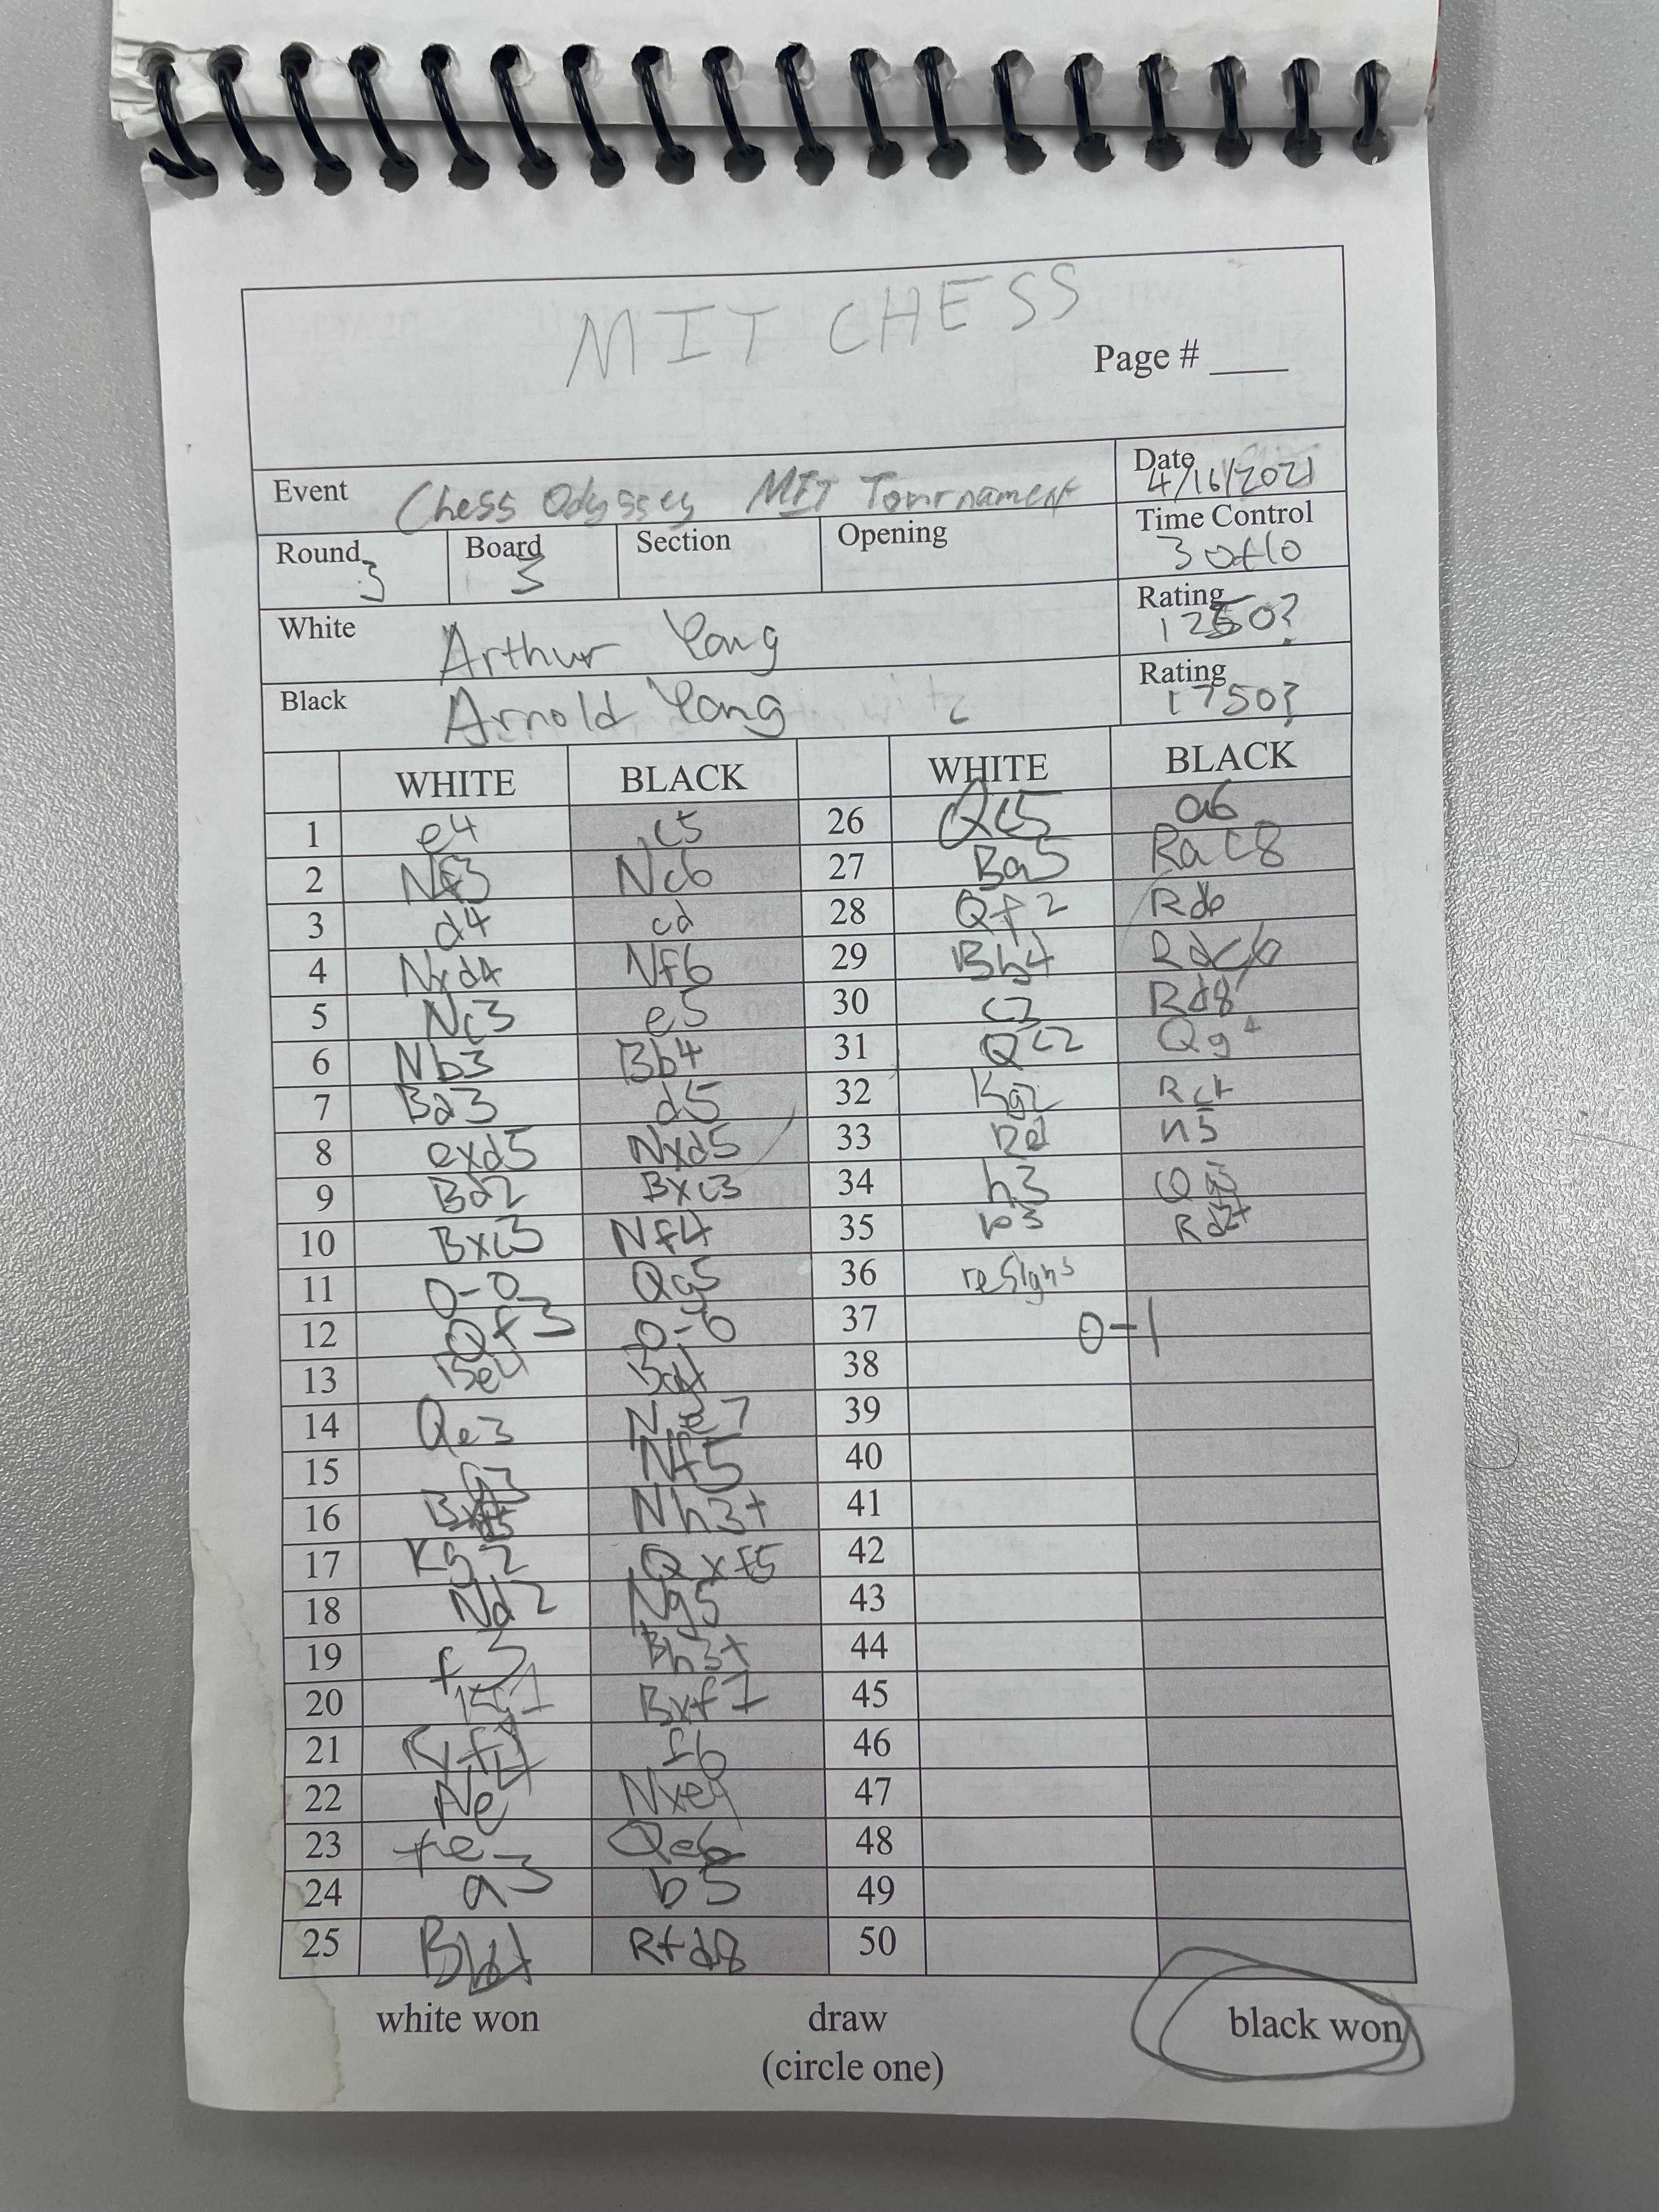
\includegraphics[width=0.75\textwidth,keepaspectratio]{images/image.png}
                \caption{Input} \pause
            \end{center}
        \end{minipage}%
        \begin{minipage}{.33\textwidth}
            \begin{center}
                \includegraphics[scale=2.0, width=0.75\textwidth,keepaspectratio]{images/box-output.png}
                \caption{Boxes} \pause
            \end{center}
        \end{minipage}
        \begin{minipage}{.33\textwidth}
            \begin{center}
                \includegraphics[width=0.75\textwidth,keepaspectratio]{images/ocr-output.png}
                \caption{OCR Output}
            \end{center}
        \end{minipage}
    \end{figure}
\end{frame}

% section 3 - how it works
\section{OCR}

\begin{frame}{Optical Character Recognition} \pause
    \begin{figure}
        \centering
        \includegraphics<2>[width=0.75\textwidth,keepaspectratio]{images/ocr-process.png}
        \includegraphics<3>[height=0.75\textheight,keepaspectratio]{images/box-output.png}
    \end{figure}
\end{frame}

\begin{frame}{Choosing a Baseline} \pause
    \begin{itemize}
        \item Tesseract \pause
        \item Kraken \pause
        \item EasyOCR
    \end{itemize}
\end{frame}

\begin{frame}{Training} \pause
    \begin{figure}
        \begin{enumerate}
            \item Transformation - TPS \pause
            \item Feature Extraction - ResNet \pause
            \item Sequence Modeling - BiLSTM \pause
            \item Prediction - Attn \pause
        \end{enumerate}
        \includegraphics[width=\textwidth]{images/framework.png}
        \caption{Four Stage STR Framework (Clova AI, 2019)}
    \end{figure}
\end{frame}

% section 4 - how it works
\section{Results}

\begin{frame}{Training Results} \pause
    \begin{figure}
        \begin{minipage}{0.5\textwidth}
            \centering
            \includegraphics[width=\textwidth,keepaspectratio]{images/demo-eval.png}
            \caption{Testing Set Demo} \pause
        \end{minipage}
        \begin{minipage}{0.5\textwidth}
            \centering
            \includegraphics[scale=2.0, width=\textwidth,keepaspectratio]{images/demo-other.png}
            \caption{Other Set Demo}
        \end{minipage}
    \end{figure}
\end{frame}

\begin{frame}{OCR Results} \pause
    \begin{figure}
        \begin{minipage}{.33\textwidth}
            \begin{center}
                \includegraphics[width=0.75\textwidth,keepaspectratio]{images/ocr-output.png}
                \caption{Version 1} \pause
            \end{center}
        \end{minipage}%
        \begin{minipage}{.33\textwidth}
            \begin{center}
                \includegraphics[width=0.75\textwidth,keepaspectratio]{images/ocr-output2.png}
                \caption{Version 2} \pause
            \end{center}
        \end{minipage}%
        \begin{minipage}{.33\textwidth}
            \begin{center}
                \includegraphics[width=0.75\textwidth,keepaspectratio]{images/ocr-output3.png}
                \caption{Version 3} \pause
            \end{center}
        \end{minipage}
    \end{figure}
\end{frame}

% section 5 - takeaways
\section{Bibliography}

\begin{frame}{Bibliography}
    \begin{enumerate}
        \item Saxena, N. (2020, August 25). PyTorch: Scene Text Detection and Recognition by CRAFT and a Four-Stage Network. Medium. https://towardsdatascience.com/pytorch-scene-text-detection-and-recognition-by-craft-and-a-four-stage-network-ec814d39db05
        \item Clova AI. (2019, December 18). \textit{What Is Wrong With Scene Text Recognition Model Comparisons? Dataset and Model Analysis.}
        \item Wikipedia. (n.d.). Thin plate spline. Wikipedia. Retrieved July 29, 2024, from https://en.wikipedia.org/wiki/Thin\_plate\_spline
        \item Wikipedia. (n.d.). Residual neural network. Wikipedia. Retrieved July 29, 2024, from https://en.wikipedia.org/wiki/Residual\_neural\_network
        \item Nama, A. (2023, May 18). Understanding Bidirectional LSTM for Sequential Data Processing. Medium. https://medium.com/@anishnama20/understanding-bidirectional-lstm-for-sequential-data-processing-b83d6283befc
    \end{enumerate}
\end{frame}

\end{document}